%\documentclass[11pt,a4paper]{article}
\documentclass[12pt,a4paper]{scrartcl}
%\documentclass[11pt,a4paper,oneside]{book}
% ===================== PACKAGES =====================
\usepackage[british]{babel}
\usepackage[tmargin=1in, bmargin=1in, lmargin=0.75in, rmargin=0.75in]{geometry}
\usepackage[dvipsnames,table]{xcolor}  % prima di tikz, listings, ecc.

\usepackage{tikz}
\usepackage{graphicx}
\usepackage{pgfplots}
\pgfplotsset{width=12cm, compat=1.9}
\usepackage{setspace}
\usepackage{chemmacros}
\usepackage{chemfig}
\usepackage{esint}
\usepackage{tabularray}
\usepackage{makeidx}
\usepackage{epstopdf}
\usepackage{amssymb}
\usepackage{mathrsfs}
\usepackage{bm}
\usepackage{amsmath}
\usepackage{enumitem}
\usepackage[english]{varioref}
\usepackage{lipsum}
\usepackage{fancyhdr}
\usepackage{float}
\usepackage{empheq}
\usepackage[framemethod=tikz]{mdframed}
\numberwithin{equation}{section}
\usepackage{eso-pic}
\usepackage{calc}
\usepackage{nccmath}
\usepackage{caption}
\usepackage{subcaption}
\usepackage{gensymb}
\usepackage{amsfonts, amsthm, epsfig, epstopdf, titling, url, array}
\usepackage{tabularx}
\usepackage{makecell}
\usepackage{booktabs}
\usepackage{array}
\usepackage{siunitx}
\sisetup{input-digits=0123456789\pi}
\usepackage[symbol]{footmisc}
\usepackage{multicol}
\usepackage{boondox-cal}
\usepackage{blindtext}
\usepackage{changepage}
\usepackage{nomencl}
\usepackage{hyperref}
\usepackage{xurl}
\usepackage{ragged2e}
\usepackage[version=4]{mhchem}  % ← conflitto di opzioni
\usepackage{longtable}
\usepackage{chemformula}
\usetikzlibrary{arrows.meta,positioning,calc}

% ===================== SI UNITS =====================
\DeclareSIUnit\atm{atm}
\DeclareSIUnit{\var}{var}
\DeclareSIUnit{\pu}{p.u.}


% ===================== MATH OPERATORS =====================
\DeclareMathOperator{\rank}{rank}
\DeclareMathOperator{\atantwo}{atan2}
\DeclareMathOperator{\spn}{span}

% ===================== COMMANDS =====================
\newcommand{\abs}[1]{\left|#1\right|}
\newcommand{\sign}{\text{sign}}
\newcommand{\centered}[1]{\begin{tabular}{@{}l@{}} #1 \end{tabular}}

% ===================== COLORS =====================
\definecolor{mycolor1}{rgb}{0.97, 0.97, 0.97}
\definecolor{mycolor2}{rgb}{0.97, 0.97, 0.97}
\definecolor{tableShade}{gray}{0.9}

% ===================== THEOREM ENVIRONMENTS =====================
\theoremstyle{it}
\newtheorem{defn}{Definition}[section]
\newtheorem{assumption}{Assumption}[section]
\newtheorem{thm}{Theorem}[section]
\newtheorem{lemma}{Lemma}[section]
\newtheorem{corollary}{Corollary}[section]
\theoremstyle{definition}
\newtheorem{example}{Example}[section]

% ===================== CUSTOM ENVIRONMENTS =====================
\newenvironment{myitemize_1}{
	\begin{itemize}[topsep=0pt]
		\setlength{\topsep}{2pt}
		\setlength{\itemsep}{2pt}
		\setlength{\parskip}{2pt}
		\setlength{\parsep}{2pt}
	}{\end{itemize}}

\newmdenv[
innerlinewidth=0.5pt,
roundcorner=4pt,
backgroundcolor=mycolor2,
linecolor=mycolor1,
innerleftmargin=6pt,
innerrightmargin=6pt,
innertopmargin=6pt,
innerbottommargin=6pt
]{mybox}

% ===================== TABLE COLUMN TYPES =====================
\newcolumntype{Y}{>{\hsize=2\hsize}X}
\newcolumntype{Z}{>{\centering\arraybackslash\hsize=0.857\hsize}X}

% ===================== SECTION DEPTH =====================
\setcounter{secnumdepth}{3}
\setcounter{tocdepth}{3}

% ===================== PAGE STYLE =====================
\setlength{\headheight}{20pt}
\setlength{\headsep}{20pt}

\pagestyle{fancy}
\fancypagestyle{firstpage}{\rhead{}}
\fancyhead[L]{\slshape\nouppercase{\leftmark}}
\chead{}
\rhead{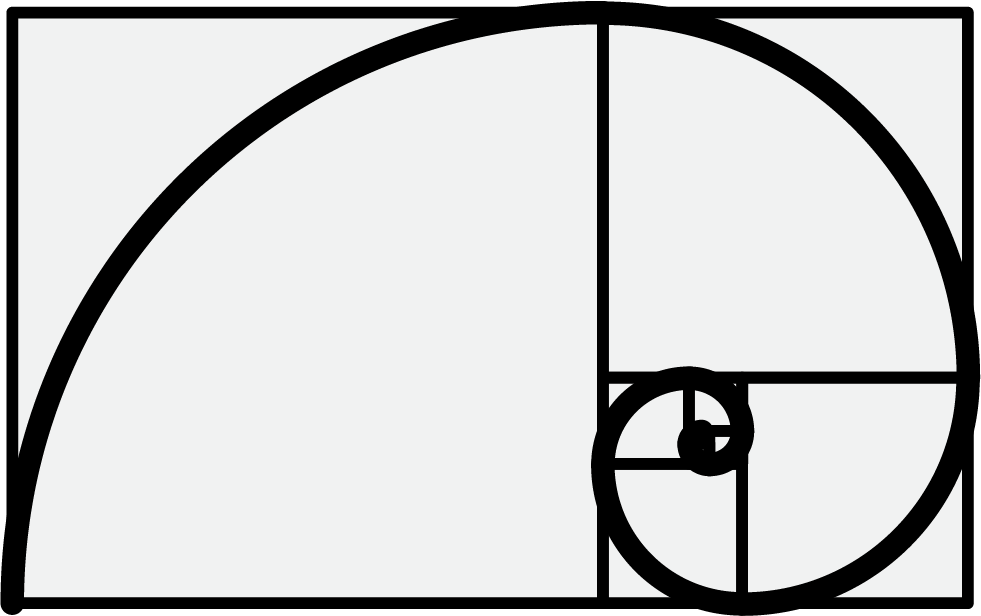
\includegraphics[height=0.75cm]{../../AAA_template_latex_settings/pwr-control_logo_doc.png}}
\lfoot{\href{http://www.pwr-control.com}{pwr-control.com}}
\cfoot{-\ \thepage\ -}
\rfoot{\textit{}}
\renewcommand{\headrulewidth}{0.4pt}
\renewcommand{\footrulewidth}{0.4pt}


\geometry{
	a4paper,
	top    = 2.5cm,
	bottom = 3.0cm,
	left   = 2.5cm,
	right  = 2.5cm
}

\hypersetup{
	colorlinks = true,
	urlcolor   = blue,
	linkcolor  = black,
	citecolor  = black
}

\pagenumbering{gobble}

% =============================================================
%  
% =============================================================

\newcommand{\DocCategory}{Technical Research Report}
\newcommand{\DocField}{Power Electronics and Control Systems}

\newcommand{\DocTitle}{%
	{\fontsize{24}{24}\selectfont\bfseries Flexible Shaft:} \\[16pt]
	{\fontsize{16}{20}\selectfont\bfseries model derivation and Simscape implementation.}
}

\newcommand{\DocSubtitle}{%
	Mechanical model for Simscape implementation
}

\newcommand{\DocAuthor}{Davide Bagnara}
\newcommand{\DocDate}{October 2022}

\newcommand{\DocAbstract}{%
	The two-mass torsional model is a standard lumped-parameter representation of a flexible shaft coupling a driving inertia to a load. Two rotational masses connected by a torsional spring and damper give rise to a single resonant mode whose frequency and damping ratio are determined by the shaft stiffness and the inertia ratio. The model is derived from Newton's second law and expressed in state-space form, yielding a fourth-order plant with a pair of lightly damped poles and a transmission zero that produces an anti-resonance in the load-side torque response.
	The transfer function from drive torque to load speed is analysed in the frequency domain, and the sensitivity of the resonance frequency to shaft geometry and material properties is examined. The model serves as the basis for active damping control design, where feedback of the torsional velocity difference between the two masses is shown to increase effective damping without affecting the rigid-body gain. Application contexts include variable-speed electric drives, hydrostatic transmissions, and any powertrain in which shaft compliance interacts with the closed-loop bandwidth of the speed or torque regulator.
}

% Tre righe metadati in fondo (label small caps + valore)
\newcommand{\MetaLabelA}{Project Repository}
\newcommand{\MetaValueA}{https://github.com/pwr-control/modelization-and-control.git}
\newcommand{\MetaValueAUrl}{https://github.com/pwr-control/modelization-and-control.git}
\newcommand{\MetaValueALabel}{modelization-and-control.git}

\newcommand{\MetaLabelB}{Framework}
\newcommand{\MetaValueB}{MATLAB/Simulink/Simscape}

\newcommand{\MetaLabelC}{Architecture}
\newcommand{\MetaValueC}{SiC, EiceDRIVER, Customized Power Supplies}

% =============================================================
%  FRONTESPIZIO
% =============================================================
\begin{document}
	\titlepage
	% ---- Intestazione centrata ----
	\begin{center}
		{\Large\scshape \DocCategory}\\[8pt]
		{\large\scshape \DocField}
	\end{center}
	
	\vspace{36pt}
	\noindent\rule{\linewidth}{0.8pt}
	
	% ---- Titolo ----
	\vspace{16pt}
	\begin{center}
		\DocTitle
	\end{center}
	
	\vspace{4pt}
	\noindent\rule{\linewidth}{2.2pt}
	
	% ---- Sottotitolo ----
	%\vspace{14pt}
	\begin{center}
		\begin{onehalfspace}
			{\large\itshape \DocSubtitle}
		\end{onehalfspace}
	\end{center}
	
	% ---- Spazio prima di Autore/Data ----
	\vspace{18pt}
	
	% ---- Author / Date su due colonne ----
	\begin{minipage}{0.92\linewidth}
		\noindent
		\begin{minipage}[t]{0.48\linewidth}
			\textbf{Author:}\\[2pt]
			\DocAuthor
		\end{minipage}%
		\hfill
		\begin{minipage}[t]{0.48\linewidth}
			\raggedleft
			\textbf{Date:}\\[2pt]
			\DocDate
		\end{minipage}
	\end{minipage}
	% ---- Spazio prima dell'abstract ----
	\vspace{36pt}
	
	% ---- Abstract indentato ----
	\begin{center}
		\begin{minipage}{0.85\linewidth}
			%    \small
			\footnotesize 
			\begin{onehalfspace}
				\textbf{Abstract:} \DocAbstract
			\end{onehalfspace}
		\end{minipage}
	\end{center}
	
	% ---- Spazio prima dei metadati ----
	\vfill
	
	% ---- Metadati in fondo ----
	\noindent
	\begin{tabular}{@{} r @{\quad} l @{}}
%		\textsc{\MetaLabelA:} & {\url{\MetaValueA}} \\[3pt]
		\textsc{\MetaLabelA:} & {\href{\MetaValueAUrl}{\MetaValueALabel}} \\[3pt]
		\textsc{\MetaLabelB:} & {\MetaValueB}       \\[3pt]
%		\textsc{\small\MetaLabelC:} & {\small\MetaValueC}       \\
	\end{tabular}
	
	% =============================================================
	%  Fine frontespizio
	% =============================================================
	\newpage
	\pagenumbering{arabic}
	\setcounter{page}{1}
	\tableofcontents
	\listoffigures	
	\listoftables
	\newpage
	
\begin{onehalfspace}
\section{Equivalent mathematical model}
The mass-spring-mass model is a valid approximation of the flexible shaft and it will be used to modelize it and its extrapolation to a generic simplified gear.
Figure \ref{figure_cranckshaft} shows a generic flexible shaft where $\tau_m$ 
is the torque actuated by a primer mover and $\tau_l$ is assumed to be a disturbance or a generic unknown load 
torque.
\subsection{Model Derivation} 
The model presents two rotational inertia masses ($J_m, J_l$) connected by a torsional spring ($k_{\vartheta}$) which include a friction term ($b_{\vartheta}$). Both two masses are connected to the chassis by two virtual bearings modeled with two simple viscosity coefficients: $b_m$ and $b_l$.

Mathematical model can be derived using Euler-Lagrange equations as follows
\begin{equation}\label{elagrange_1}
	\frac{d}{dt}\left(\frac{\partial E_{kin}}{\partial \dot{q}_1} \right) - 
	\frac{\partial E_{kin}}{\partial q_1} + \frac{\partial E_{pot}}{\partial 
		q_1} =\underbrace{Q_{diss}^{(12)} + Q_1}_\text{not conservative force}
\end{equation}
\begin{equation}\label{elagrange_2}
	\frac{d}{dt}\left(\frac{\partial E_{kin}}{\partial \dot{q}_2} \right) - 
	\frac{\partial E_{kin}}{\partial q_2} + \frac{\partial E_{pot}}{\partial 
		q_2} = \underbrace{Q_{diss}^{(21)} + Q_2}_\text{not conservative force}
\end{equation}
\begin{figure}[H]
	\centering
	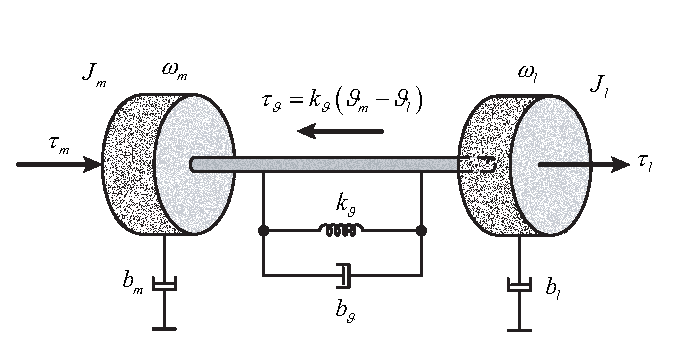
\includegraphics[width = 320pt, keepaspectratio] {figures/msm/flexshaft_1.eps}
	\captionsetup{width=0.5\textwidth}		
	\caption{Generic flexible shaft model.}
	\label{figure_cranckshaft}
\end{figure}
Where $Q_1$, $Q_2$, $Q_{diss}^{(12)}$ and $Q_{diss}^{(21)}$ are the generalized 
forces, like magnetic force, unknown load, disturbance and  friction or in general not conservative force\footnote{A conservative force is a force which is derive by a potential and satisfies to the following conditions:
	\begin{flalign}
		\vec{\nabla}\times\vec{f}=\vec{0} &&
	\end{flalign}
	\begin{flalign}
		\oint_{\mathscr{C}}\vec{f}\cdot d\vec{r}=0 &&
	\end{flalign}
	\begin{flalign}
		\vec{f}=-\vec{\nabla}\phi &&
	\end{flalign}
}. 

Applying Eqs.~\eqref{elagrange_1} and~\eqref{elagrange_2} for the case
\begin{equation}
	\begin{aligned}
		q_1&=\vartheta_m \\[6pt]	
		q_2&=\vartheta_l
	\end{aligned}
\end{equation}
The kinematic and potential energy can be written as follows
\begin{equation}
	E_{kin} = \frac{1}{2}J_m\dot{\vartheta}_m^2 + \frac{1}{2}J_l\dot{\vartheta}_l^2
\end{equation}
\begin{equation}
	E_{pot} = \frac{1}{2}k_{\vartheta}\left(\vartheta_m-\vartheta_l\right)^2
\end{equation}

Applying the Lagrange equations we obtain the following motion equations
\begin{flalign}
	J_m\ddot{\vartheta}_m+k_{\vartheta}\left( \vartheta_m-\vartheta_l\right)  &= 
	-b_m\dot{\vartheta}_m-b_{\vartheta}\left(\dot{\vartheta}_m-\dot{\vartheta_l}\right) + 
	\tau_m \\[6pt]
	J_l\ddot{\vartheta}_l-k_{\vartheta}\left( \vartheta_m-\vartheta_l\right)  &= 
	-b_l\dot{\vartheta}_l-b_{\vartheta}\left(\dot{\vartheta_l}-\dot{\vartheta}_m\right) + 
	\tau_l
\end{flalign}
or 
\begin{equation}
	\left\lbrace \begin{aligned}
		\dot{\vartheta}_m &= \omega_m \\[6pt]
		\dot{\omega}_m &= 
		-\frac{k_{\vartheta}}{J_m}\vartheta_m-\frac{b_m+b_{\vartheta}}{J_m}\omega_m 
		+\frac{k_{\vartheta}}{J_m}\vartheta_l+\frac{b_{\vartheta}}{J_m}\omega_l+\frac{1}{J_m}\tau_m
		\\[6pt]
		\dot{\vartheta}_l &= \omega_l \\[6pt]
		\dot{\omega}_l &= 
		\frac{k_{\vartheta}}{J_l}\vartheta_m+\frac{b_{\vartheta}}{J_l}\omega_m-\frac{k_{\vartheta}}{J_l}\vartheta_l-\frac{b_l+b_{\vartheta}}{J_l}\omega_l
		+\frac{1}{J_l}\tau_l
	\end{aligned}\right. 
\end{equation}
The state space representation become
\begin{equation}
	\dot{\vec{z}} = \tilde{\mathbf{G}}\vec{z}+\tilde{\mathbf{H}} \ 
	\tau_m+\tilde{\mathbf{M}} \ \tau_l
\end{equation}
where $\vec{z}=\left[ \begin{matrix}
	\vartheta_m&\omega_m&\vartheta_l&\omega_l
\end{matrix}\right]^T$
and 
\begin{equation}
	\tilde{\mathbf{G}} = 
	\left[ \begin{matrix}
		0&1&0&0\\[6pt]
		-\frac{k_{\vartheta}}{J_m}&-\frac{b_m+b_{\vartheta}}{J_m}&\frac{k_{\vartheta}}{J_m}&\frac{b_{\vartheta}}{J_m}\\[6pt]
		0&0&0&1\\[6pt]
		\frac{k_{\vartheta}}{J_l}&\frac{b_{\vartheta}}{J_l}&-\frac{k_{\vartheta}}{J_l}&-\frac{b_l+b_{\vartheta}}{J_l}
	\end{matrix}\right]
\end{equation}
and $\tilde{\mathbf{H}} =\left[ \begin{matrix}
	0&\frac{1}{J_m}&0&0
\end{matrix}\right]^T$, 
$\tilde{\mathbf{M}} =\left[ \begin{matrix}
	0&0&0&-\frac{1}{J_l}
\end{matrix}\right]^T$.

For our purpose, we want to change the state representation using a new state 
vector 
\begin{equation}
	\vec{x} = \mathbf{T}\vec{z} = \begin{bmatrix} \omega_m \\[6pt] \omega_l \\[6pt] \tau_{\vartheta} \end{bmatrix}
\end{equation}
where\footnote{where 
	\begin{flalign}
		\tau_{\vartheta}=k_\vartheta(\vartheta_m-\vartheta_l) &&
	\end{flalign} 
	which can be written also as 
	\begin{flalign}
		\dot{\tau}_{\vartheta}=k_\vartheta(\omega_m-\omega_l) &&
	\end{flalign} 
	which describes the dynamic of the shaft torsional torque.} $\mathbf{T}$ is 
given by\footnote{the matrix pseudo inverse has been used.}
\begin{equation}
	\mathbf{T} = \left[\begin{matrix}
		0 & 1 & 0 & 0 \\[6pt]
		0 & 0 & 0 & 1 \\[6pt]
		k_{\vartheta} & 0 & -k_{\vartheta} & 0
	\end{matrix}\right]
	\quad \text{and} \quad
	\mathbf{T}^{-1} = \left[\begin{matrix}
		0 & 0 & \frac{1}{2k_{\vartheta}} \\[6pt]
		1 & 0 & 0 \\[6pt]
		0 & 0 & -\frac{1}{2k_{\vartheta}} \\[6pt]
		0 & 1 & 0
	\end{matrix}\right]
\end{equation}
Basically, the linear transformation $\mathbf{T}$ consists in a model reduction. The minimum representation of a dynamical system can be reached applying some matrix analysis results, but also considering the total number of energy storage which are contained into the system. In the case of mass-spring-mass model, we can assume that three components can store energy: the two inertial masses $J_m$ and $J_l$ as kinetic energy, and the torsional spring as potential energy. That means the minimal representation of the mass-spring-mass model is made by three equations.

The new state space representation becomes
\begin{flalign}
	\dot{\vec{z}} &= \tilde{\mathbf{G}}\vec{z}+\tilde{\mathbf{H}} \ 
	\tau_1+\tilde{\mathbf{M}} \ \tau_2 \\[6pt]
	\mathbf{T}^{-1}\dot{\vec{x}} &= 
	\tilde{\mathbf{G}}\mathbf{T}^{-1}\vec{x}+\tilde{\mathbf{H}} \ 
	\tau_1+\tilde{\mathbf{M}} \ \tau_2 \\[6pt]
	%&\vdots \\
	\dot{\vec{x}} &= 
	\mathbf{T}\tilde{\mathbf{G}}\mathbf{T}^{-1}\vec{x}+\mathbf{T}\tilde{\mathbf{H}}
	\ \tau_1+\mathbf{T}\tilde{\mathbf{M}} \ \tau_2
\end{flalign}
or
\begin{mybox}
	\begin{equation}
		\dot{\vec{x}} = \tilde{\mathbf{A}}\vec{x}+\tilde{\mathbf{B}}\,\tau_1+\tilde{\mathbf{E}}\,\tau_2
	\end{equation}
	or
	\begin{equation}\label{two_mass_2}
		\left[ \begin{matrix}
			\dot{\omega}_m \\[6pt]
			\dot{\omega}_l \\[6pt]
			\dot{\tau_{\vartheta}}
		\end{matrix}\right] = 
		\left[ \begin{matrix}
			-\frac{b_m+b_{\vartheta}}{J_m} & \frac{b_{\vartheta}}{J_m} & 
			-\frac{1}{J_m}\\[6pt]
			\frac{b_{\vartheta}}{J_l} & -\frac{b_l+b_{\vartheta}}{J_l} & 
			\frac{1}{J_l}\\[6pt]
			k_{\vartheta} & -k_{\vartheta} & 0
		\end{matrix}\right]
		\left[ \begin{matrix}
			{\omega_m} \\[6pt]
			{\omega_l} \\[6pt]
			{\tau_{\vartheta}}
		\end{matrix}\right] + 
		\left[ \begin{matrix}
			\frac{1}{J_m} \\[6pt]
			0 \\[6pt]
			0
		\end{matrix}\right] \tau_m+
		\left[ \begin{matrix}
			0 \\[6pt]
			\frac{1}{J_l} \\[6pt]
			0
		\end{matrix}\right] \tau_l
	\end{equation}
	where 
	
	\begin{equation*}
		\vec{x} = \left[\begin{matrix} \omega_m&\omega_l&\tau_{\vartheta} 
		\end{matrix} \right]^T
	\end{equation*}
	
	\begin{equation*}
		\tilde{\mathbf{A}} = \mathbf{T}\tilde{\mathbf{G}}\mathbf{T}^{-1} =
		\left[ \begin{matrix}
			-\frac{b_m+b_{\vartheta}}{J_m} & \frac{b_{\vartheta}}{J_m} & 
			-\frac{1}{J_m}\\[6pt]
			\frac{b_{\vartheta}}{J_l} & -\frac{b_l+b_{\vartheta}}{J_l} & 
			\frac{1}{J_l}\\[6pt]
			k_{\vartheta} & -k_{\vartheta} & 0
		\end{matrix}\right]
	\end{equation*}
	
	\begin{equation*}
		\tilde{\mathbf{B}} = \mathbf{T}\tilde{\mathbf{H}} =
		\left[ \begin{matrix}
			\frac{1}{J_m} \\[6pt]
			0 \\[6pt]
			0
		\end{matrix}\right]
		\quad
		\tilde{\mathbf{E}} = \mathbf{T}\tilde{\mathbf{M}} =
		\left[ \begin{matrix}
			0 \\[6pt]
			\frac{1}{J_l} \\[6pt]
			0
		\end{matrix}\right]
	\end{equation*}
	\textbf{Consider the term $\tau_l(t)$ as a disturbance (or load) which perturbs 
		the system.}
	
	\vspace{5mm}
	For a more physical viewpoint the mass-spring-mass (or flexible shaft) dynamic 
	equations can also be written as follows:
	\begin{equation}
		\left\lbrace 
		\begin{aligned}
			& \dot{\omega}_m =\frac{1}{J_m}\Big[ -\big(b_m+b_\vartheta\big)\omega_m+b_{\vartheta}\omega_l - \tau_{\vartheta} + \tau_m\Big] \\[6pt]
			& \dot{\omega}_l = \frac{1}{J_l}\Big[b_\vartheta\omega_m-\big(b_l+b_{\vartheta}\big)\omega_l+ 
			\tau_{\vartheta} + \tau_l\Big] \\[6pt]
			& \dot{\tau}_{\vartheta} = k_{\vartheta}\big(\omega_m-\omega_l\big) 
		\end{aligned}
		\right. 
	\end{equation}
\end{mybox}

\subsection{Natural oscillations}
The frequency of the natural oscillation of the shaft can be evaluated imposing to zero the friction terms and calculating the eigenvalue of the transition matrix, as follows

\noindent setting $b_m=0$,  $b_l=0$ and $b_\vartheta=0$ we obtain the following characteristic polynomial
\begin{equation}\label{eigenvalues_msm}
	\Big|s\mathbf{I}-\tilde{\mathbf{A}}\Big|=\begin{vmatrix}
		s & 0 & 1/J_m \\[6pt]
		0 & s & -1/J_l \\[6pt]
		-k_\vartheta & k_\vartheta & s 
	\end{vmatrix} = s\Big[s^2+k_\vartheta\frac{J_m+J_l}{J_mJ_l}\Big]
\end{equation}
setting $s=j\omega$ to the Eq.~\eqref{eigenvalues_msm} and equating to zero
\begin{equation}
	\omega^2-k_\vartheta\frac{J_m+J_l}{J_mJ_l}=0
\end{equation}
we obtain
\begin{equation}
		\omega_0=\sqrt{k_\vartheta\frac{J_m+J_l}{J_mJ_l}}
\end{equation}
which represent the pulsation of the natural harmonic component of the system.

\section{Extension to a generic gear model}
The mathematical structure of the flexible shaft can be used also to develop a simplified gear.

Let
\begin{equation}
	\omega_l=\omega_m/n_{tg}
\end{equation}
be the relation between driver (m) and follower (l) speeds, where $\omega_l$ is the follower speed and $\omega_m$ is the driver speed. The term $n_{tg}$ represents the ratio between the driver and the follower speeds of the gear.

The mathematical model of the simplified gear is here represented ($b_\vartheta=0$ is assumed), 
\begin{equation}\left\lbrace 
	\begin{aligned}
		\dot{\omega}_m &= \frac{1}{J_m}\Big[\tau_m - \tau_\vartheta^m - b_m\omega_m\Big] \\[8pt]
		\dot{\omega}_l &= \frac{1}{J_l}\Big[\tau_\vartheta^l + \tau_l - b_l\omega_l \Big] \\[8pt]
		\dot{\tau}_\vartheta^m &= k_\vartheta\Big[\omega_m -\omega_l n_{tg} \Big] \\[8pt]
		n_{tg} &= \frac{n_m}{n_l} \\[8pt]
		\tau_\vartheta^m &=\frac{\tau_\vartheta^l}{n_{tg}}
	\end{aligned}\right. 
\end{equation}
where $\tau_\vartheta^m$ is the torsional torque seen at the driver side as well as $\tau_\vartheta^l$ is the torsional torque seen at the follower side, see also Figure~\ref{figure_gear_flexshaft}.
\begin{figure}[H]
	\centering
	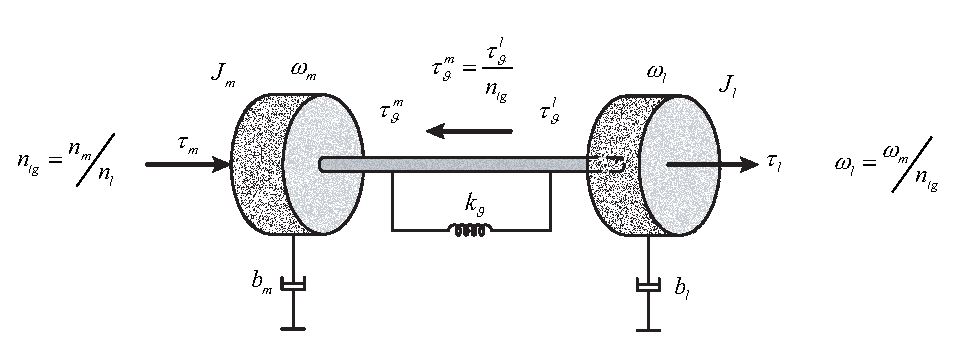
\includegraphics[width = 400pt, keepaspectratio] {figures/msm/gear_flexshaft_2.eps}
	\captionsetup{width=0.5\textwidth}		
	\caption{Generic flexible gear-shaft model.}
	\label{figure_gear_flexshaft}
\end{figure}

\section{Flexible Shaft - Model parameters settings}
Parameters setting consist of
\begin{itemize}
	\item[--] $J_m\quad\Big[\SI{}{\kilo\gram\square\meter}\Big]$: Inertia of the \textit{m}-side rotating mass.
	\item[--] $J_l\quad\Big[\SI{}{\kilo\gram\square\meter}\Big]$: Inertia of the \textit{l}-side rotating mass.
	\item[--] $b_m\quad\Big[\SI{}{\newton\second\per\radian}\Big]$: Friction coefficient - \textit{m}-side.
	\item[--] $b_l\quad\Big[\SI{}{\newton\second\per\radian}\Big]$: Friction coefficient - \textit{l}-side.
	\item[--] $k_\vartheta\quad\Big[\SI{}{\newton\per\radian}\Big]$: Internal torsional spring.	
	\item[--] $b_\vartheta\quad\Big[\SI{}{\newton\second\per\radian}\Big]$: Damping of the internal torsional spring.
\end{itemize}

\section{Gear - Model parameters settings}
Parameters setting consist of
\begin{itemize}
	\item[--] $n_m\quad\Big[\SI{}{ad}\Big]$: with $n_l$ forms the gear ratio $n_{tg} = \frac{n_m}{n_l}$.
	\item[--] $n_l\quad\Big[\SI{}{ad}\Big]$: with $n_m$ forms the gear ratio $n_{tg} = \frac{n_m}{n_l}$.
	\item[--] $J_m\quad\Big[\SI{}{\kilo\gram\square\meter}\Big]$: Inertia of the \textit{driver}-side rotating mass.
	\item[--] $J_l\quad\Big[\SI{}{\kilo\gram\square\meter}\Big]$: Inertia of the \textit{follower}-side rotating mass.
	\item[--] $b_m\quad\Big[\SI{}{\newton\second\per\radian}\Big]$: Friction coefficient - \textit{driver}-side.
	\item[--] $b_l\quad\Big[\SI{}{\newton\second\per\radian}\Big]$: Friction coefficient - \textit{follower}-side.
	\item[--] $k_\vartheta\quad\Big[\SI{}{\newton\per\radian}\Big]$: Internal torsional spring.	
\end{itemize}
\end{onehalfspace}

\end{document} 